% =============================================================================
% CHAPITRE 1 - CINÉMATIQUE
% Partie 9 : Mouvement d'un projectile
% Version maritime pour l'IMQ
% =============================================================================

% =============================================================================
\section{Mouvement d'un projectile}
% =============================================================================
\subsection*{Un peu d'histoire : Galilée et la décomposition du mouvement}

Avant \textbf{Galilée} (1564--1642), les savants croyaient qu'un boulet de canon suivait d'abord une ligne droite, puis tombait verticalement une fois sa « force » épuisée. Cette vision, héritée d'Aristote, ne correspondait pas aux observations.

La contribution révolutionnaire de Galilée fut de comprendre que \textbf{le mouvement horizontal et le mouvement vertical sont indépendants}. Un objet lancé continue d'avancer horizontalement \emph{en même temps} qu'il tombe verticalement --- les deux mouvements se superposent sans s'influencer mutuellement.

\begin{remarque}[title=Le principe d'indépendance des mouvements]
Galilée démontra ce principe par une expérience de pensée : une bille lâchée du haut du mât d'un navire en mouvement tombe au pied du mât, pas derrière. La bille conserve le mouvement horizontal du navire pendant sa chute.

Ce principe est fondamental pour les navigateurs : un objet qui tombe d'un navire en mouvement ne tombe pas « en arrière » --- il conserve la vitesse du navire.
\end{remarque}

Cette décomposition en mouvements indépendants est la clé pour analyser les projectiles : on traite séparément la direction horizontale (mouvement uniforme) et la direction verticale (chute libre), puis on combine les résultats.

\vspace{0.5cm}

Un \textbf{projectile} est un objet lanc\'e dans l'air qui se d\'eplace ensuite uniquement sous l'influence de la gravit\'e. C'est l'application directe des principes du mouvement en 2D que nous venons de voir.

\begin{remarque}[title=Questions types que nous allons r\'esoudre]
Dans cette section, vous apprendrez \`a r\'epondre aux questions suivantes :
\begin{itemize}
    \item Quelle est la \textbf{port\'ee} (distance horizontale) d'un projectile?
    \item Quelle \textbf{hauteur maximale} atteint-il?
    \item Combien de \textbf{temps} reste-t-il en l'air?
    \item O\`u \textbf{atterrit} un objet lanc\'e horizontalement?
    \item \`A quel angle faut-il lancer pour atteindre une cible?
    \item O\`u tombe un objet l\^ach\'e d'un navire en mouvement?
\end{itemize}
\end{remarque}

\begin{definition}[title=Projectile]
Un projectile est un corps lanc\'e avec une vitesse initiale quelconque et qui se d\'eplace sous la seule action de la gravit\'e (r\'esistance de l'air n\'eglig\'ee).

Exemples : ballon lanc\'e, balle de baseball, fus\'ee \'eclairante, lance-amarre, boulet de canon.
\end{definition}

\begin{attention}[title=Rappel fondamental]
Puisque la gravit\'e est la \textbf{seule force} et qu'elle agit \textbf{verticalement} :
\begin{itemize}
    \item En $x$ : pas d'acc\'el\'eration ($a_x = 0$) $\Rightarrow$ \textbf{MRU}
    \item En $y$ : acc\'el\'eration constante ($a_y = -g$) $\Rightarrow$ \textbf{Chute libre}
\end{itemize}
La composante horizontale de la vitesse \textbf{reste constante} tout au long du vol!
\end{attention}

\subsection{Strat\'egie de r\'esolution}

\begin{remarque}[title=Strat\'egie de r\'esolution -- TR\`ES IMPORTANT]
Pour r\'esoudre des probl\`emes de projectile en 2D, il faut \textbf{toujours} :
\begin{enumerate}
    \item \textbf{D\'ecomposer} le mouvement en deux directions : $x$ (horizontal) et $y$ (vertical)
    \item \textbf{Traiter s\'epar\'ement} chaque direction
    \item \textbf{Relier} les deux directions par le \textbf{temps} $\Delta t$ (qui est le m\^eme pour les deux)
\end{enumerate}
\end{remarque}

\begin{center}
\begin{tikzpicture}[scale=0.9]
% Axes
\draw[axe, thick, ->] (0,0) -- (8,0) node[right] {$x$};
\draw[axe, thick, ->] (0,0) -- (0,5) node[above] {$y$};
% Trajectoire
\draw[very thick, blue, domain=0:7, samples=50] plot (\x, {3*\x/7 + 0.5 - 0.12*\x*\x});
% Positions
\foreach \t in {0,1,2,3,4,5,6,7} {
    \pgfmathsetmacro{\ypos}{3*\t/7 + 0.5 - 0.12*\t*\t}
    \fill[blue] (\t, \ypos) circle (3pt);
}
% Vecteurs vitesse
\draw[thick, red, ->] (0,0.5) -- (1,0.93) node[above right] {\small $\vec{v}_0$};
\draw[thick, red, ->] (3.5,2.03) -- (4.5,1.89);
\draw[thick, red, ->] (7,0.5) -- (8,-0.36);
% Composantes à t=0
\draw[thick, green!60!black, ->] (0,0.5) -- (1,0.5) node[below] {\small $v_{0x}$};
\draw[thick, orange, ->] (0,0.5) -- (0,0.93) node[left] {\small $v_{0y}$};
% Annotations
\node at (3.5,4) {\textbf{Trajectoire parabolique}};
\node[blue] at (3.5,-0.5) {En $x$ : MRU ($v_x$ constante)};
\node[blue] at (3.5,-1) {En $y$ : Chute libre ($a_y = -g$)};
\end{tikzpicture}
\end{center}

\subsection{Décomposition de la vitesse initiale}

Si le projectile est lancé avec une vitesse initiale $v_0$ faisant un angle $\theta$ avec l'horizontale :

\begin{equationimportante}
\textbf{Composantes de la vitesse initiale}
\begin{align}
v_{0x} &= v_0 \cos\theta \\[0.2cm]
v_{0y} &= v_0 \sin\theta
\end{align}
\end{equationimportante}

\begin{center}
\begin{tikzpicture}[scale=1.2]
% Axes
\draw[axe, thick, ->] (0,0) -- (4,0) node[right] {$x$};
\draw[axe, thick, ->] (0,0) -- (0,3) node[above] {$y$};
% Vecteur v0
\draw[very thick, red, ->] (0,0) -- (3,2) node[above right] {$\vec{v}_0$};
% Composantes
\draw[thick, green!60!black, ->] (0,0) -- (3,0) node[below] {$v_{0x} = v_0 \cos\theta$};
\draw[thick, orange, ->] (3,0) -- (3,2) node[right] {$v_{0y} = v_0 \sin\theta$};
% Angle
\draw[thick] (0.8,0) arc (0:33.7:0.8) node[midway, right] {$\theta$};
% Valeur de v0
\node at (1.2,1.3) {$v_0$};
\end{tikzpicture}
\end{center}

\subsection{Équations du mouvement}

\begin{center}
\renewcommand{\arraystretch}{1.8}
\begin{tabular}{|c|c|}
\hline
\rowcolor{bleuclair}
\textbf{Direction horizontale ($x$)} & \textbf{Direction verticale ($y$)} \\
\hline
MRU (vitesse constante) & Chute libre (MRUA) \\
\hline
$a_x = 0$ & $a_y = -g$ \\
\hline
$v_x = v_{0x} = v_0 \cos\theta$ & $v_y = v_{0y} - g\Delta t = v_0 \sin\theta - g\Delta t$ \\
\hline
$\Delta x = v_{0x} \Delta t = (v_0 \cos\theta) \Delta t$ & $\Delta y = v_{0y} \Delta t - \dfrac{1}{2}g(\Delta t)^2$ \\
\hline
& $v_y^2 = v_{0y}^2 - 2g\Delta y$ \\
\hline
\end{tabular}
\end{center}

\begin{remarque}[title=Le temps relie les deux directions]
Le temps $\Delta t$ est \textbf{le même} pour le mouvement horizontal et vertical. C'est ce qui permet de relier les deux directions et de résoudre les problèmes.
\end{remarque}

\subsection{Caract\'eristiques de la trajectoire}

Lors de l'analyse d'un projectile, on s'int\'eresse souvent \`a trois grandeurs cl\'es. Plut\^ot que de m\'emoriser des formules sp\'ecifiques, il est pr\'ef\'erable de comprendre \textbf{comment les trouver} \`a partir des \'equations de base.

\begin{center}
\begin{tikzpicture}[scale=0.9]
% Axes
\draw[axe, thick, ->] (0,0) -- (9,0) node[right] {$x$};
\draw[axe, thick, ->] (0,0) -- (0,5) node[above] {$y$};

% Trajectoire parabolique (portée = 7, h_max = 3.5)
\draw[very thick, blue, domain=0:7, samples=100] plot (\x, {2*\x - 2*\x*\x/7});

% Point de départ
\fill[red] (0,0) circle (4pt);
\node[below left] at (0,0) {D\'epart};

% Point d'arrivée
\fill[red] (7,0) circle (4pt);
\node[below right] at (7,0) {Arriv\'ee};

% Point au sommet (à x = 3.5, y = 3.5)
\fill[green!60!black] (3.5,3.5) circle (4pt);
\node[above] at (3.5,3.8) {Sommet};

% Hauteur maximale
\draw[<->, thick, green!60!black] (3.5,0) -- (3.5,3.5);
\node[right, green!60!black] at (3.6,1.75) {$h_{max}$};
\draw[dashed, gray] (0,3.5) -- (3.5,3.5);

% Portée
\draw[<->, thick, orange] (0,-0.7) -- (7,-0.7);
\node[below, orange] at (3.5,-0.7) {Port\'ee};

% Vecteur vitesse initiale
\draw[very thick, red, ->] (0,0) -- (1.2,1.5) node[above left] {$\vec{v}_0$};
\draw[thick] (0.5,0) arc (0:51:0.5);
\node at (0.85,0.35) {$\theta$};

% Vecteur vitesse au sommet (horizontal)
\draw[very thick, red, ->] (3.5,3.5) -- (4.7,3.5) node[above] {$\vec{v}$};
\node[below] at (4.5,3.2) {\small ($v_y = 0$)};

% Vecteur vitesse finale
\draw[very thick, red, ->] (7,0) -- (8.2,-1.5);

% Temps de montée et descente
\draw[<->, thick, purple] (0,4.3) -- (3.5,4.3);
\node[above, purple] at (1.75,4.3) {\small $t_{mont\acute{e}e}$};
\draw[<->, thick, purple] (3.5,4.3) -- (7,4.3);
\node[above, purple] at (5.25,4.3) {\small $t_{descente}$};

% Annotation temps total
\node[below] at (3.5,-1.4) {Temps de vol total : $\Delta t = t_{mont\acute{e}e} + t_{descente}$};

\end{tikzpicture}
\end{center}

\begin{remarque}[title=Observations importantes sur le sch\'ema]
\begin{itemize}
    \item Au \textbf{sommet}, la vitesse n'est \textbf{pas nulle}! Seule la composante verticale $v_y$ est nulle. La composante horizontale $v_x$ reste constante tout au long du vol.
    \item Pour un projectile lanc\'e et retombant au m\^eme niveau, le temps de mont\'ee \'egale le temps de descente (sym\'etrie).
    \item La trajectoire est une \textbf{parabole}, cons\'equence directe du MRU en $x$ et du MRUA en $y$.
\end{itemize}
\end{remarque}

\subsubsection{Port\'ee horizontale}

\begin{definition}[title=Port\'ee]
La \textbf{port\'ee} est la distance horizontale totale parcourue par le projectile entre son lancement et son atterrissage.
\end{definition}

\textbf{Comment la trouver :}
\begin{enumerate}
    \item D\'eterminer le \textbf{temps de vol} $\Delta t$ en utilisant l'\'equation verticale (quand $y$ revient au niveau d'arriv\'ee)
    \item Utiliser ce temps dans l'\'equation horizontale : $\text{Port\'ee} = v_{0x} \cdot \Delta t$
\end{enumerate}

\begin{remarque}
Pour un projectile lanc\'e et retombant au m\^eme niveau, la port\'ee est maximale lorsque l'angle de lancement est de $45^\circ$.
\end{remarque}

\subsubsection{Hauteur maximale}

\begin{definition}[title=Hauteur maximale]
La \textbf{hauteur maximale} est l'altitude la plus \'elev\'ee atteinte par le projectile au cours de son vol.
\end{definition}

\textbf{Comment la trouver :}

Au point le plus haut, la composante verticale de la vitesse s'annule ($v_y = 0$). On utilise alors l'\'equation $v_y^2 = v_{0y}^2 - 2g\Delta y$ avec $v_y = 0$ pour trouver $\Delta y_{max}$.

\subsubsection{Temps de vol}

\begin{definition}[title=Temps de vol]
Le \textbf{temps de vol} est la dur\'ee totale pendant laquelle le projectile reste en l'air, du lancement jusqu'\`a l'atterrissage.
\end{definition}

\textbf{Comment le trouver :}

On utilise l'\'equation de position verticale $\Delta y = v_{0y} \Delta t - \frac{1}{2}g(\Delta t)^2$ en fixant $\Delta y$ \'egal au d\'eplacement vertical total (souvent z\'ero si retour au m\^eme niveau, ou n\'egatif si atterrissage plus bas).

\begin{attention}[title=Approche recommand\'ee]
Plut\^ot que de m\'emoriser des formules sp\'ecifiques pour la port\'ee, la hauteur maximale ou le temps de vol, il est beaucoup plus efficace de :
\begin{enumerate}
    \item Ma\^itriser les \'equations de base (MRU en $x$, chute libre en $y$)
    \item Identifier ce qu'on cherche et ce qu'on conna\^it
    \item Appliquer la strat\'egie de d\'ecomposition syst\'ematiquement
\end{enumerate}
Cette approche fonctionne pour \textbf{tous} les probl\`emes de projectile, m\^eme les plus complexes!
\end{attention}

\subsection{Exemples}

\begin{exemple}{Ballon de soccer (exemple terrestre)}{ballon-soccer}
Un joueur botte un ballon avec une vitesse initiale de $\SI{20}{m/s}$ \`a un angle de $30^\circ$ par rapport au sol.
\begin{enumerate}[label=\alph*)]
    \item Quelle est la port\'ee du tir?
    \item Quelle hauteur maximale atteint le ballon?
    \item Combien de temps le ballon reste-t-il en l'air?
\end{enumerate}

\textbf{Donn\'ees :}
\begin{itemize}
    \item $v_0 = \SI{20}{m/s}$, $\theta = 30^\circ$
    \item $v_{0x} = 20 \cos 30^\circ = \SI{17,3}{m/s}$
    \item $v_{0y} = 20 \sin 30^\circ = \SI{10}{m/s}$
\end{itemize}

\textbf{b) Hauteur maximale :} (on commence par celle-ci car elle ne n\'ecessite pas le temps)

Au point le plus haut, $v_y = 0$. Utilisons $v_y^2 = v_{0y}^2 - 2g\Delta y$ :
\begin{align*}
0 &= 10^2 - 2(9,81)\Delta y_{max} \\
\Delta y_{max} &= \frac{100}{19,62} = \SI{5,10}{m}
\end{align*}

\textbf{c) Temps de vol :}

Le ballon revient au sol quand $\Delta y = 0$. Utilisons $\Delta y = v_{0y} \Delta t - \frac{1}{2}g(\Delta t)^2$ :
\begin{align*}
0 &= 10 \Delta t - 4,905(\Delta t)^2 \\
0 &= \Delta t (10 - 4,905 \Delta t)
\end{align*}

Solutions : $\Delta t = 0$ (d\'epart) ou $\Delta t = \frac{10}{4,905} = \SI{2,04}{s}$ (atterrissage)

\textbf{a) Port\'ee :}

Maintenant qu'on conna\^it le temps de vol :
\[ \text{Port\'ee} = v_{0x} \cdot \Delta t = 17,3 \times 2,04 = \SI{35,3}{m} \]
\end{exemple}

\begin{exemple}{Lance-amarre (exemple maritime)}{lance-amarre}
Un marin utilise un lance-amarre pour envoyer une ligne vers un quai. L'appareil lance le projectile à $\SI{25}{m/s}$ avec un angle de $40^\circ$. Le marin se trouve sur le pont à $\SI{6}{m}$ au-dessus du niveau du quai.

Quelle est la portée horizontale du tir?

\textbf{Données :}
\begin{itemize}
    \item $v_0 = \SI{25}{m/s}$, $\theta = 40^\circ$
    \item $y_i = \SI{6}{m}$, $y_f = \SI{0}{m}$ (niveau du quai)
    \item $v_{0x} = 25 \cos 40^\circ = \SI{19,2}{m/s}$
    \item $v_{0y} = 25 \sin 40^\circ = \SI{16,1}{m/s}$
\end{itemize}

\textbf{Étape 1 : Trouver le temps de vol}

On utilise l'équation en $y$ :
\begin{align*}
y_f &= y_i + v_{0y} \Delta t - \frac{1}{2}g(\Delta t)^2 \\
0 &= 6 + 16,1 \Delta t - 4,905(\Delta t)^2
\end{align*}

Équation quadratique : $4,905(\Delta t)^2 - 16,1\Delta t - 6 = 0$

\[ \Delta t = \frac{16,1 + \sqrt{259,2 + 117,7}}{9,81} = \frac{16,1 + 19,4}{9,81} = \SI{3,62}{s} \]

\textbf{Étape 2 : Calculer la portée}
\[ \Delta x = v_{0x} \Delta t = 19,2 \times 3,62 = \SI{69,5}{m} \]

Le lance-amarre peut atteindre une cible à environ $\SI{70}{m}$.

\begin{remarque}
Le fait de lancer depuis une position surélevée augmente significativement la portée par rapport à un lancer au niveau du sol.
\end{remarque}
\end{exemple}

\begin{pratiqueautonome}
Un lance-amarre tire une ligne avec une vitesse initiale de $\SI{30}{m/s}$ à un angle de $40^\circ$ au-dessus de l'horizontale, depuis une hauteur de $\SI{4}{m}$ au-dessus de l'eau.

\begin{enumerate}[label=\alph*)]
    \item Décomposez la vitesse initiale en ses composantes $v_{0x}$ et $v_{0y}$.
    \item Calculez la portée horizontale (distance où la ligne touche l'eau).
\end{enumerate}

\textit{Indice : Trouvez d'abord le temps de vol en résolvant $y_f = 0$.}

\espaceresolution[8cm]
\reponsepratique{a) $v_{0x} \approx \SI{23,0}{m/s}$, $v_{0y} \approx \SI{19,3}{m/s}$ \quad b) Portée $\approx \SI{97}{m}$}
\end{pratiqueautonome}

\begin{exemple}{Homme à la mer depuis un navire en mouvement}{homme-a-la-mer}
Un marin tombe d'un navire qui avance à $\SI{8}{n\oe{}uds}$. Il tombe d'une hauteur de $\SI{10}{m}$. À quelle distance horizontale du point de chute le marin entre-t-il dans l'eau?

\textbf{Analyse :} Au moment de la chute, le marin a la même vitesse horizontale que le navire. C'est un projectile lancé horizontalement ($\theta = 0^\circ$).

\textbf{Conversion de la vitesse :}
\[ v_{0x} = \SI{8}{n\oe{}uds} \times \frac{\SI{0,5144}{m/s}}{\SI{1}{n\oe{}ud}} = \SI{4,1}{m/s} \]

\textbf{Données :}
\begin{itemize}
    \item $v_{0x} = \SI{4,1}{m/s}$ (vitesse du navire)
    \item $v_{0y} = \SI{0}{m/s}$ (chute, pas saut)
    \item $\Delta y = \SI{-10}{m}$
\end{itemize}

\textbf{Temps de chute :} On utilise l'équation de position verticale avec $v_{0y} = 0$ :
\begin{align*}
\Delta y &= v_{0y} \Delta t - \frac{1}{2}g(\Delta t)^2 \\
-10 &= 0 - \frac{1}{2}(9,81)(\Delta t)^2 \\
(\Delta t)^2 &= \frac{2 \times 10}{9,81} = 2,04 \\
\Delta t &= \SI{1,43}{s}
\end{align*}

\textbf{Distance horizontale :}
\[ \Delta x = v_{0x} \Delta t = 4,1 \times 1,43 = \SI{5,9}{m} \]

Le marin entre dans l'eau à environ $\SI{6}{m}$ en avant du point d'où il est tombé (par rapport à l'eau, pas par rapport au navire qui continue d'avancer).

\begin{attention}
Pendant ce temps, le navire a aussi avancé de $\SI{5,9}{m}$. Du point de vue d'un observateur sur le navire, le marin semble tomber verticalement! C'est le principe de l'indépendance des mouvements.
\end{attention}
\end{exemple}

\begin{exemple}{Probl\`eme inverse : trouver l'angle de lancement}{probleme-inverse-angle}
Un canon lance-amarre doit atteindre un quai situ\'e \`a $\SI{50}{m}$ de distance horizontale. La vitesse de sortie du projectile est de $\SI{30}{m/s}$. Le canon et le quai sont au m\^eme niveau.

\`A quel angle faut-il r\'egler le canon?

\textbf{Donn\'ees :}
\begin{itemize}
    \item Port\'ee souhait\'ee : $\Delta x = \SI{50}{m}$
    \item Vitesse initiale : $v_0 = \SI{30}{m/s}$
    \item D\'eplacement vertical : $\Delta y = 0$ (m\^eme niveau)
    \item Inconnue : $\theta = ?$
\end{itemize}

\textbf{Strat\'egie :} On doit relier la port\'ee \`a l'angle. Exprimons $\Delta x$ en fonction de $\theta$.

\textbf{\'Etape 1 : Trouver le temps de vol en fonction de $\theta$}

Quand le projectile revient au m\^eme niveau, $\Delta y = 0$ :
\begin{align*}
\Delta y &= v_{0y} \Delta t - \frac{1}{2}g(\Delta t)^2 \\
0 &= (v_0 \sin\theta) \Delta t - \frac{1}{2}g(\Delta t)^2 \\
0 &= \Delta t \left( v_0 \sin\theta - \frac{1}{2}g \Delta t \right)
\end{align*}

Solutions : $\Delta t = 0$ (d\'epart) ou $\Delta t = \dfrac{2 v_0 \sin\theta}{g}$ (atterrissage)

\textbf{\'Etape 2 : Exprimer la port\'ee}
\begin{align*}
\Delta x &= v_{0x} \cdot \Delta t = (v_0 \cos\theta) \cdot \frac{2 v_0 \sin\theta}{g} \\
\Delta x &= \frac{2 v_0^2 \sin\theta \cos\theta}{g} = \frac{v_0^2 \sin(2\theta)}{g}
\end{align*}

(On utilise l'identit\'e trigonom\'etrique $2\sin\theta\cos\theta = \sin(2\theta)$)

\textbf{\'Etape 3 : Isoler $\theta$}
\begin{align*}
\sin(2\theta) &= \frac{g \cdot \Delta x}{v_0^2} = \frac{9,81 \times 50}{30^2} = \frac{490,5}{900} = 0,545
\end{align*}

\[ 2\theta = \arcsin(0,545) = 33,0^\circ \quad \Rightarrow \quad \theta = 16,5^\circ \]

\textbf{Attention!} L'\'equation $\sin(2\theta) = 0,545$ a \textbf{deux solutions} entre $0^\circ$ et $90^\circ$ :
\begin{itemize}
    \item $2\theta = 33,0^\circ$ $\Rightarrow$ $\theta_1 = 16,5^\circ$ (tir tendu)
    \item $2\theta = 180^\circ - 33,0^\circ = 147^\circ$ $\Rightarrow$ $\theta_2 = 73,5^\circ$ (tir en cloche)
\end{itemize}

\begin{center}
\begin{tikzpicture}[scale=0.55]
% Axes
\draw[axe, thick, ->] (0,0) -- (8,0) node[right] {$x$};
\draw[axe, thick, ->] (0,0) -- (0,5) node[above] {$y$};

% Trajectoire basse (16.5$^\circ$)
\draw[very thick, blue, domain=0:7, samples=50] plot (\x, {0.42*\x - 0.03*\x*\x});
\draw[thick, blue, ->] (0,0) -- (1.4,0.42) node[above left] {\small $\theta_1 = 16,5^\circ$};

% Trajectoire haute (73.5$^\circ$)
\draw[very thick, red, domain=0:7, samples=50] plot (\x, {2.38*\x - 0.17*\x*\x});
\draw[thick, red, ->] (0,0) -- (0.42,1.4) node[above left] {\small $\theta_2 = 73,5^\circ$};

% Point cible
\fill[green!60!black] (7,0) circle (5pt);
\node[below] at (7,0) {Cible};

% Légende
\node[blue] at (5,0.8) {\small Tir tendu};
\node[red] at (2,4) {\small Tir en cloche};
\end{tikzpicture}
\end{center}

\textbf{R\'eponse :} Deux angles sont possibles : $\theta_1 = 16,5^\circ$ ou $\theta_2 = 73,5^\circ$.

\begin{remarque}[title=Choix pratique]
En pratique, le tir tendu ($16,5^\circ$) est souvent pr\'ef\'er\'e car :
\begin{itemize}
    \item Le temps de vol est plus court (la ligne reste tendue)
    \item Le tir est moins affect\'e par le vent
    \item La pr\'ecision est g\'en\'eralement meilleure
\end{itemize}
Le tir en cloche peut \^etre utile pour passer par-dessus un obstacle.
\end{remarque}
\end{exemple}

\begin{exemple}{Port\'ee maximale impossible}{portee-maximale-impossible}
Avec le m\^eme canon ($v_0 = \SI{30}{m/s}$), peut-on atteindre une cible \`a $\SI{100}{m}$?

\textbf{V\'erification :}
\[ \sin(2\theta) = \frac{g \cdot \Delta x}{v_0^2} = \frac{9,81 \times 100}{900} = 1,09 \]

Puisque $\sin(2\theta)$ ne peut jamais d\'epasser 1, \textbf{aucun angle} ne permet d'atteindre cette cible!

\textbf{Port\'ee maximale :} Elle est atteinte quand $\sin(2\theta) = 1$, soit $\theta = 45^\circ$ :
\[ \Delta x_{max} = \frac{v_0^2}{g} = \frac{900}{9,81} = \SI{91,7}{m} \]

La cible \`a $\SI{100}{m}$ est hors de port\'ee.
\end{exemple}

\subsection{Projectile lanc\'e horizontalement}

Un cas particulier important est le projectile lancé \textbf{horizontalement} (angle $\theta = 0^\circ$).

\begin{center}
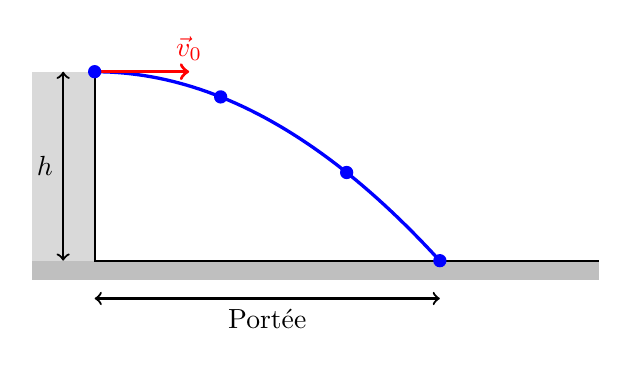
\begin{tikzpicture}[scale=0.8]
% Falaise
\fill[gray!30] (-1,3) rectangle (0,0);
\fill[gray!50] (-1,0) rectangle (8,-0.3);
\draw[thick] (0,3) -- (0,0) -- (8,0);
% Trajectoire
\draw[very thick, blue, domain=0:5.5, samples=50] plot (\x, {3 - 0.1*\x*\x});
% Vecteur vitesse initiale
\draw[very thick, red, ->] (0,3) -- (1.5,3) node[above] {$\vec{v}_0$};
% Points et vecteurs
\fill[blue] (0,3) circle (3pt);
\fill[blue] (2,2.6) circle (3pt);
\fill[blue] (4,1.4) circle (3pt);
\fill[blue] (5.48,0) circle (3pt);
% Hauteur
\draw[<->, thick] (-0.5,0) -- (-0.5,3) node[midway, left] {$h$};
% Portée
\draw[<->, thick] (0,-0.6) -- (5.48,-0.6) node[midway, below] {Portée};
\end{tikzpicture}
\end{center}

Dans ce cas :
\begin{itemize}
    \item $v_{0x} = v_0$ (toute la vitesse est horizontale)
    \item $v_{0y} = 0$ (pas de composante verticale initiale)
\end{itemize}

Le temps de chute s'obtient à partir de l'équation de position verticale. Avec $v_{0y} = 0$ et $\Delta y = -h$ :
\[ \Delta y = -\frac{1}{2}g(\Delta t)^2 \quad \Rightarrow \quad (\Delta t)^2 = \frac{2h}{g} \quad \Rightarrow \quad \Delta t = \sqrt{\frac{2h}{g}} \]

La portée s'obtient ensuite par le MRU horizontal :
\[ \text{Portée} = v_0 \cdot \Delta t \]

\begin{exemple}{Conteneur tombant d'une grue}{conteneur-chute-grue}
Un conteneur se détache d'une grue portuaire en mouvement. La grue se déplace horizontalement à $\SI{2}{m/s}$ et le conteneur est à $\SI{15}{m}$ de hauteur.

À quelle distance horizontale (par rapport au point de largage) le conteneur touche-t-il le sol?

\textbf{Données :} $v_{0x} = \SI{2}{m/s}$, $v_{0y} = 0$, $\Delta y = \SI{-15}{m}$

\textbf{Temps de chute :} Avec $v_{0y} = 0$, l'équation de position verticale donne :
\begin{align*}
\Delta y &= -\frac{1}{2}g(\Delta t)^2 \\
-15 &= -\frac{1}{2}(9,81)(\Delta t)^2 \\
(\Delta t)^2 &= \frac{30}{9,81} = 3,06 \\
\Delta t &= \SI{1,75}{s}
\end{align*}

\textbf{Distance horizontale :}
\[ \Delta x = v_{0x} \cdot \Delta t = 2 \times 1,75 = \SI{3,5}{m} \]

Le conteneur touche le sol à $\SI{3,5}{m}$ du point situé directement sous la position de largage.
\end{exemple}

\subsection{Résumé : stratégie de résolution}

\begin{remarque}[title=Méthode pour résoudre un problème de projectile]
\begin{enumerate}
    \item \textbf{Dessiner} un schéma avec les axes $x$ et $y$
    \item \textbf{Décomposer} la vitesse initiale : $v_{0x} = v_0 \cos\theta$, $v_{0y} = v_0 \sin\theta$
    \item \textbf{Identifier} les données et l'inconnue
    \item \textbf{Choisir} les équations appropriées (souvent, trouver $\Delta t$ en premier)
    \item \textbf{Résoudre} en traitant $x$ et $y$ séparément
    \item \textbf{Vérifier} que la réponse est physiquement raisonnable
\end{enumerate}
\end{remarque}